\documentclass[12pt, c]{beamer}
\setbeamersize{text margin left=5mm, text margin right=5mm}

% --- PACKAGES ---
\usepackage[utf8]{inputenc}
\usepackage[T1]{fontenc}
\usepackage{xcolor}
\usepackage{tikz}
\usetikzlibrary{decorations.pathmorphing}
\usepackage{tcolorbox}
\tcbuselibrary{skins}

%quiets meaningless errors
\usepackage{anyfontsize}

\usepackage{tikz}
\usepackage{xcolor}


%This template gives you the option of inserting distinct grainy backgrounds.
%These backgrounds all came from https://texturelabs.org/
% Usage: \usetexture[opacity]{1, 2, 3, or 4}
\newcommand{\usetexture}[2][0.25]{
    \setbeamertemplate{background canvas}{
        % 1. Fetch your preamble background color
        \usebeamercolor{background canvas}
        \begin{tikzpicture}[remember picture,overlay]
            % 2. Paint the background with your theme's color first
            \fill[background canvas.bg] (current page.south west) rectangle (current page.north east);

            % 3. Draw the texture node
            \node[inner sep=0pt, opacity=#1] at (current page.center) {
                \includegraphics[width=\paperwidth,height=\paperheight]{
                    \ifcase#2\relax \or noise1.jpg \or noise2.jpg \or noise3.jpg \or noise4.jpg \or noise5.jpg \else noise6.jpg \fi
                }
            };
        \end{tikzpicture}
    } 
}

\newcommand{\notexture}{\setbeamertemplate{background canvas}{}}


%\usepackage{beton}
\usepackage{newpxtext,newpxmath}
\usepackage{euler}

% This tells Beamer to use the fonts you actually loaded
\usefonttheme{serif} 
\usefonttheme{professionalfonts}

% --- COLOR PALETTE ---
%Best practice: Select from a palette on https://coolors.co
%click on a color on their page and it copies the HEX (HTML) data for that color
\definecolor{background1}{HTML}{2D3436}%body slide color
\definecolor{background2}{HTML}{393938}%for the environments box
\definecolor{titlepagecolor}{HTML}{232A32}%title page background
\definecolor{border1}{HTML}{ADAEA7} %for the environments box
\definecolor{maintitletext}{HTML}{FF5F15} %Striking color for the title of the presentation
\definecolor{slidetitletext}{HTML}{778DA9}%For the titles of slides
\definecolor{text1}{HTML}{F5F6FA}%main text color
\definecolor{text2}{HTML}{050A10}%for content of environments box
\definecolor{text3}{HTML}{232A32}%For title of the environments box
%for variation


% --- BEAMER SETTINGS ---
\setbeamercolor{background canvas}{bg=background1}
\setbeamercolor{normal text}{fg=text1}
\setbeamercolor{title}{fg=maintitletext}
\setbeamercolor{frametitle}{fg=maintitletext}
\setbeamerfont{frametitle}{series=\bfseries, size=\large}
\setbeamertemplate{navigation symbols}{} % Clean look

\setbeamercolor{item}{fg=maintitletext}


% 1. Define a counter to track how many boxes have been drawn
\newcounter{sketchycounter}

% --- CUSTOM "SKETCHY" BOX FOR THEOREMS ---
\newtcolorbox{sketchybox}[2][1]{
  colback=background2,
  colframe=border1,
  colupper=text2,         
  coltitle=text3,         
  fonttitle=\bfseries,
  title=#2,
  enhanced,
  boxrule=1.5pt,
  % 2. Increment the counter every time this environment is called
  code={\stepcounter{sketchycounter}},
  underlay={
    \begin{scope}
      % Clip the texture to the inside of the box
      \clip (interior.south west) rectangle (interior.north east);
      
      % 3. Calculate a modulo (0, 1, 2, or 3) based on the counter
      \pgfmathsetmacro{\noiseorient}{mod(\thesketchycounter, 4)}
      
      % 4. Assign x/y scaling based on the modulo state
      \ifcase\noiseorient\relax
          \def\xs{1}\def\ys{1}   % State 0: Normal
      \or
          \def\xs{-1}\def\ys{1}  % State 1: Flipped Horizontally
      \or
          \def\xs{1}\def\ys{-1}  % State 2: Flipped Vertically
      \or
          \def\xs{-1}\def\ys{-1} % State 3: Flipped Both (180 degree rotation)
      \fi

      % 5. Apply \xs and \ys to the node
      \node[inner sep=0pt, opacity=0.2, xscale=\xs, yscale=\ys] at (interior.center) {
          \ifcase#1\relax \or
              
\includegraphics[width=\paperwidth,height=\paperheight]{noise1light.jpg} \or
              
\includegraphics[width=\paperwidth,height=\paperheight]{noise2light.jpg} \or
              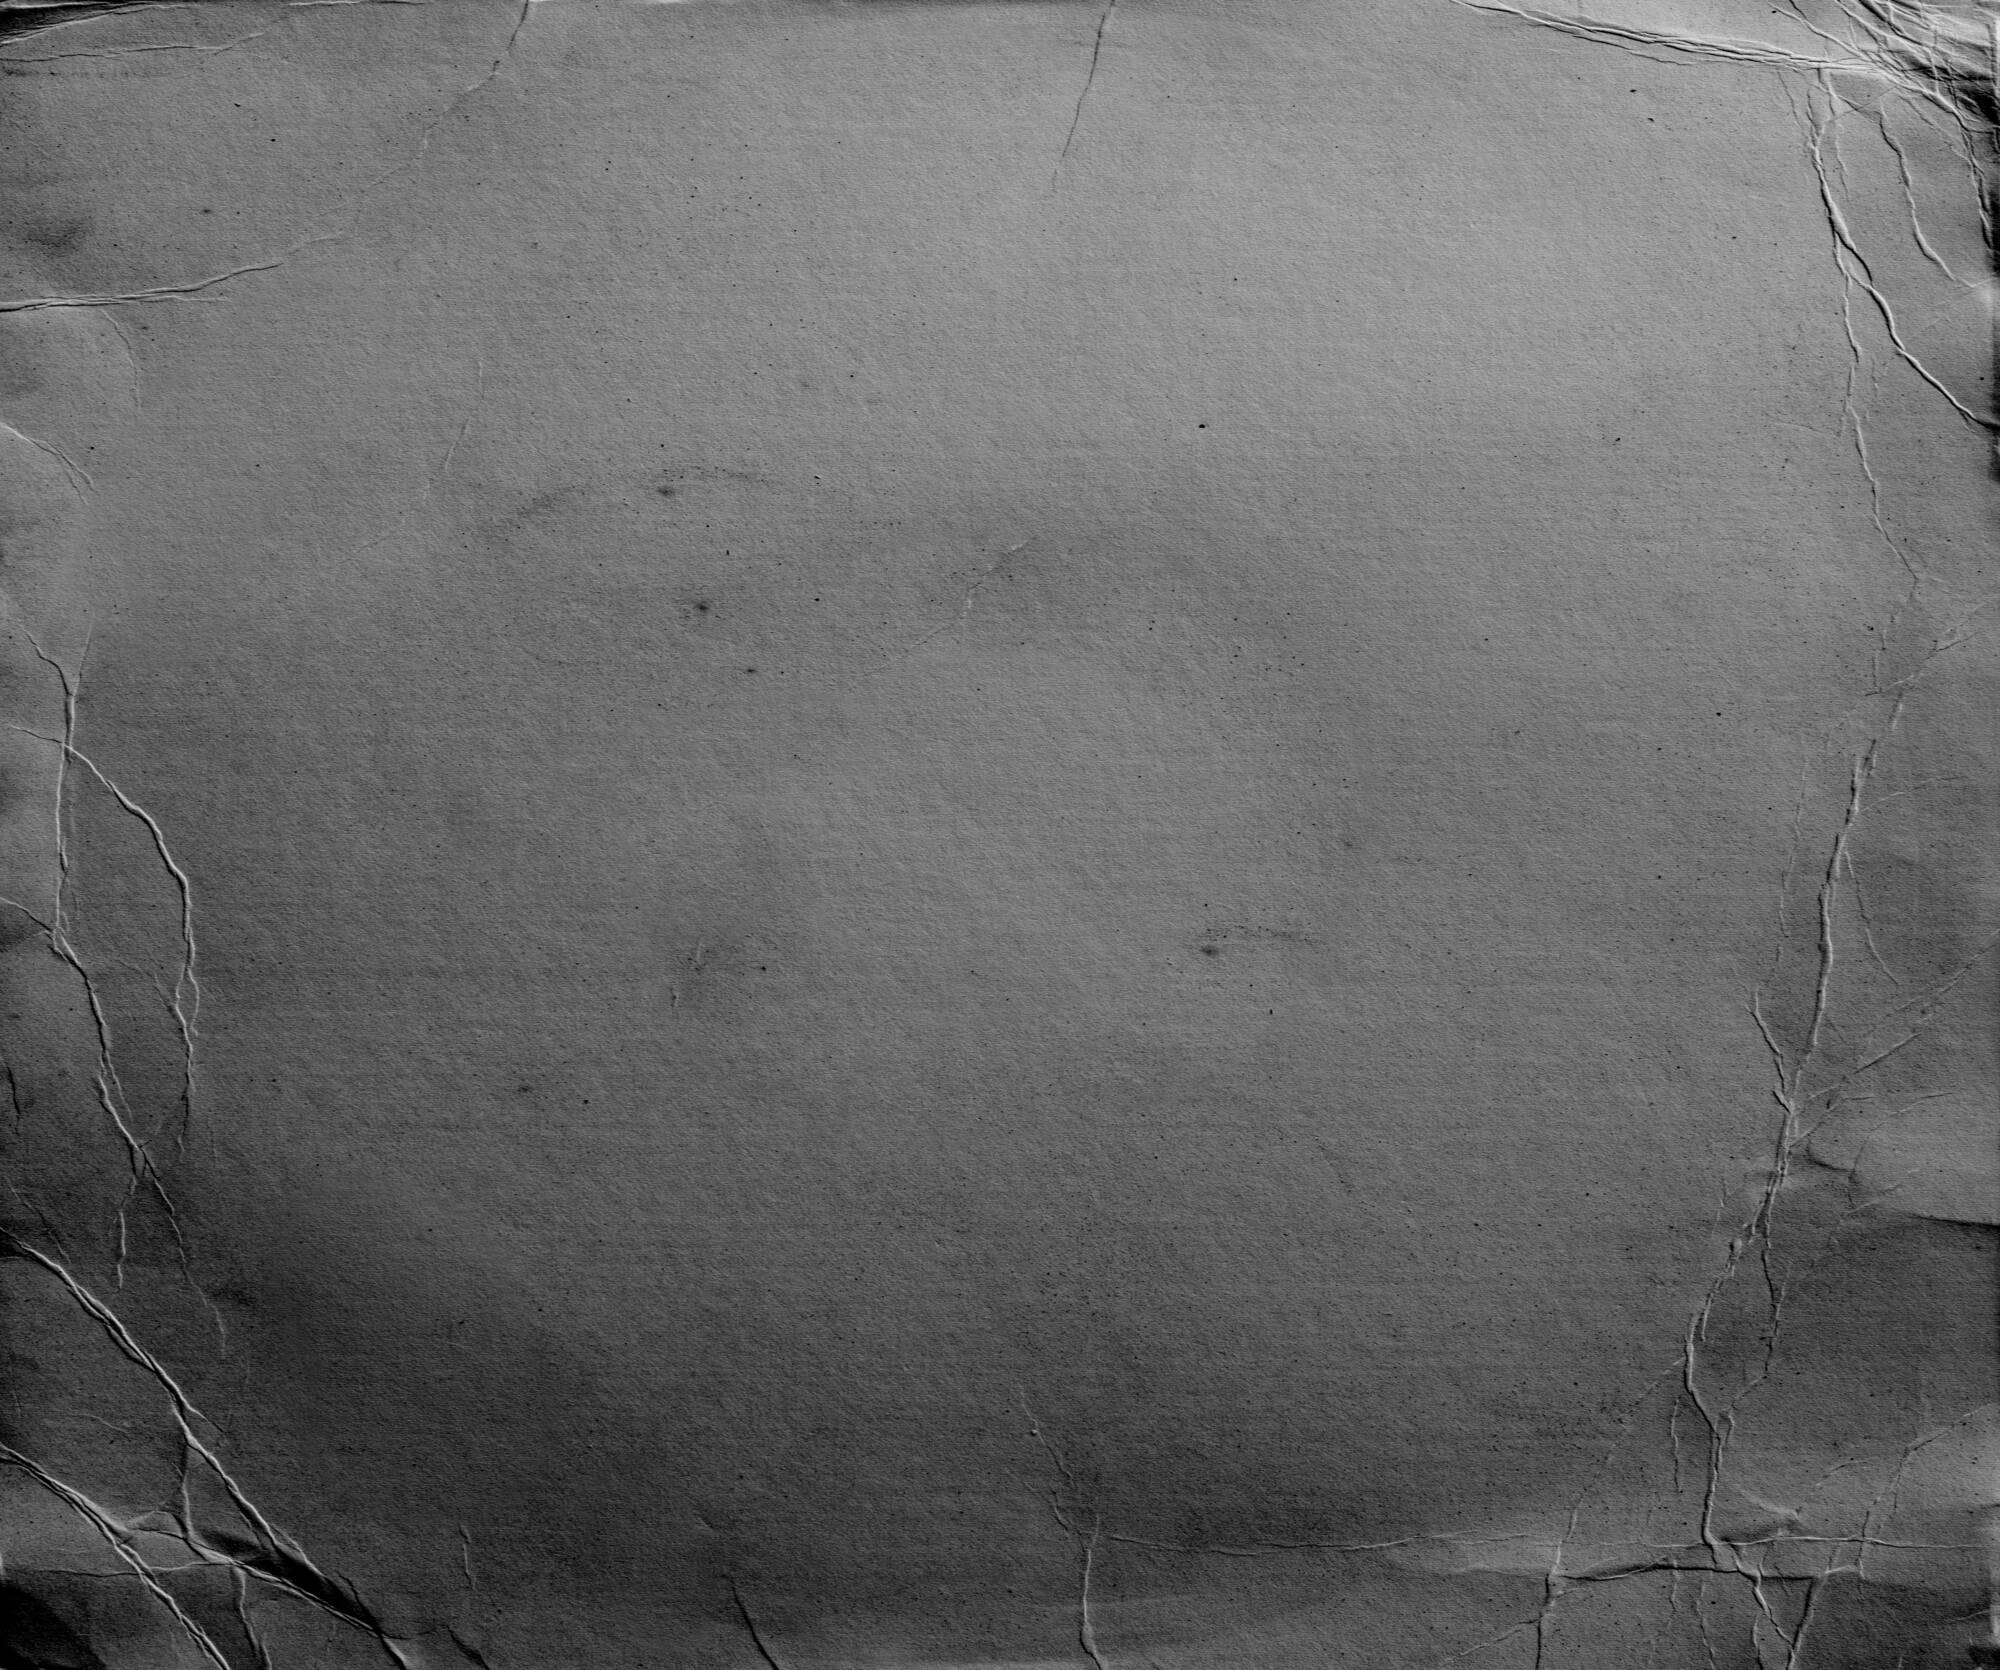
\includegraphics[width=\paperwidth,height=\paperheight]{noise3.jpg} \or
              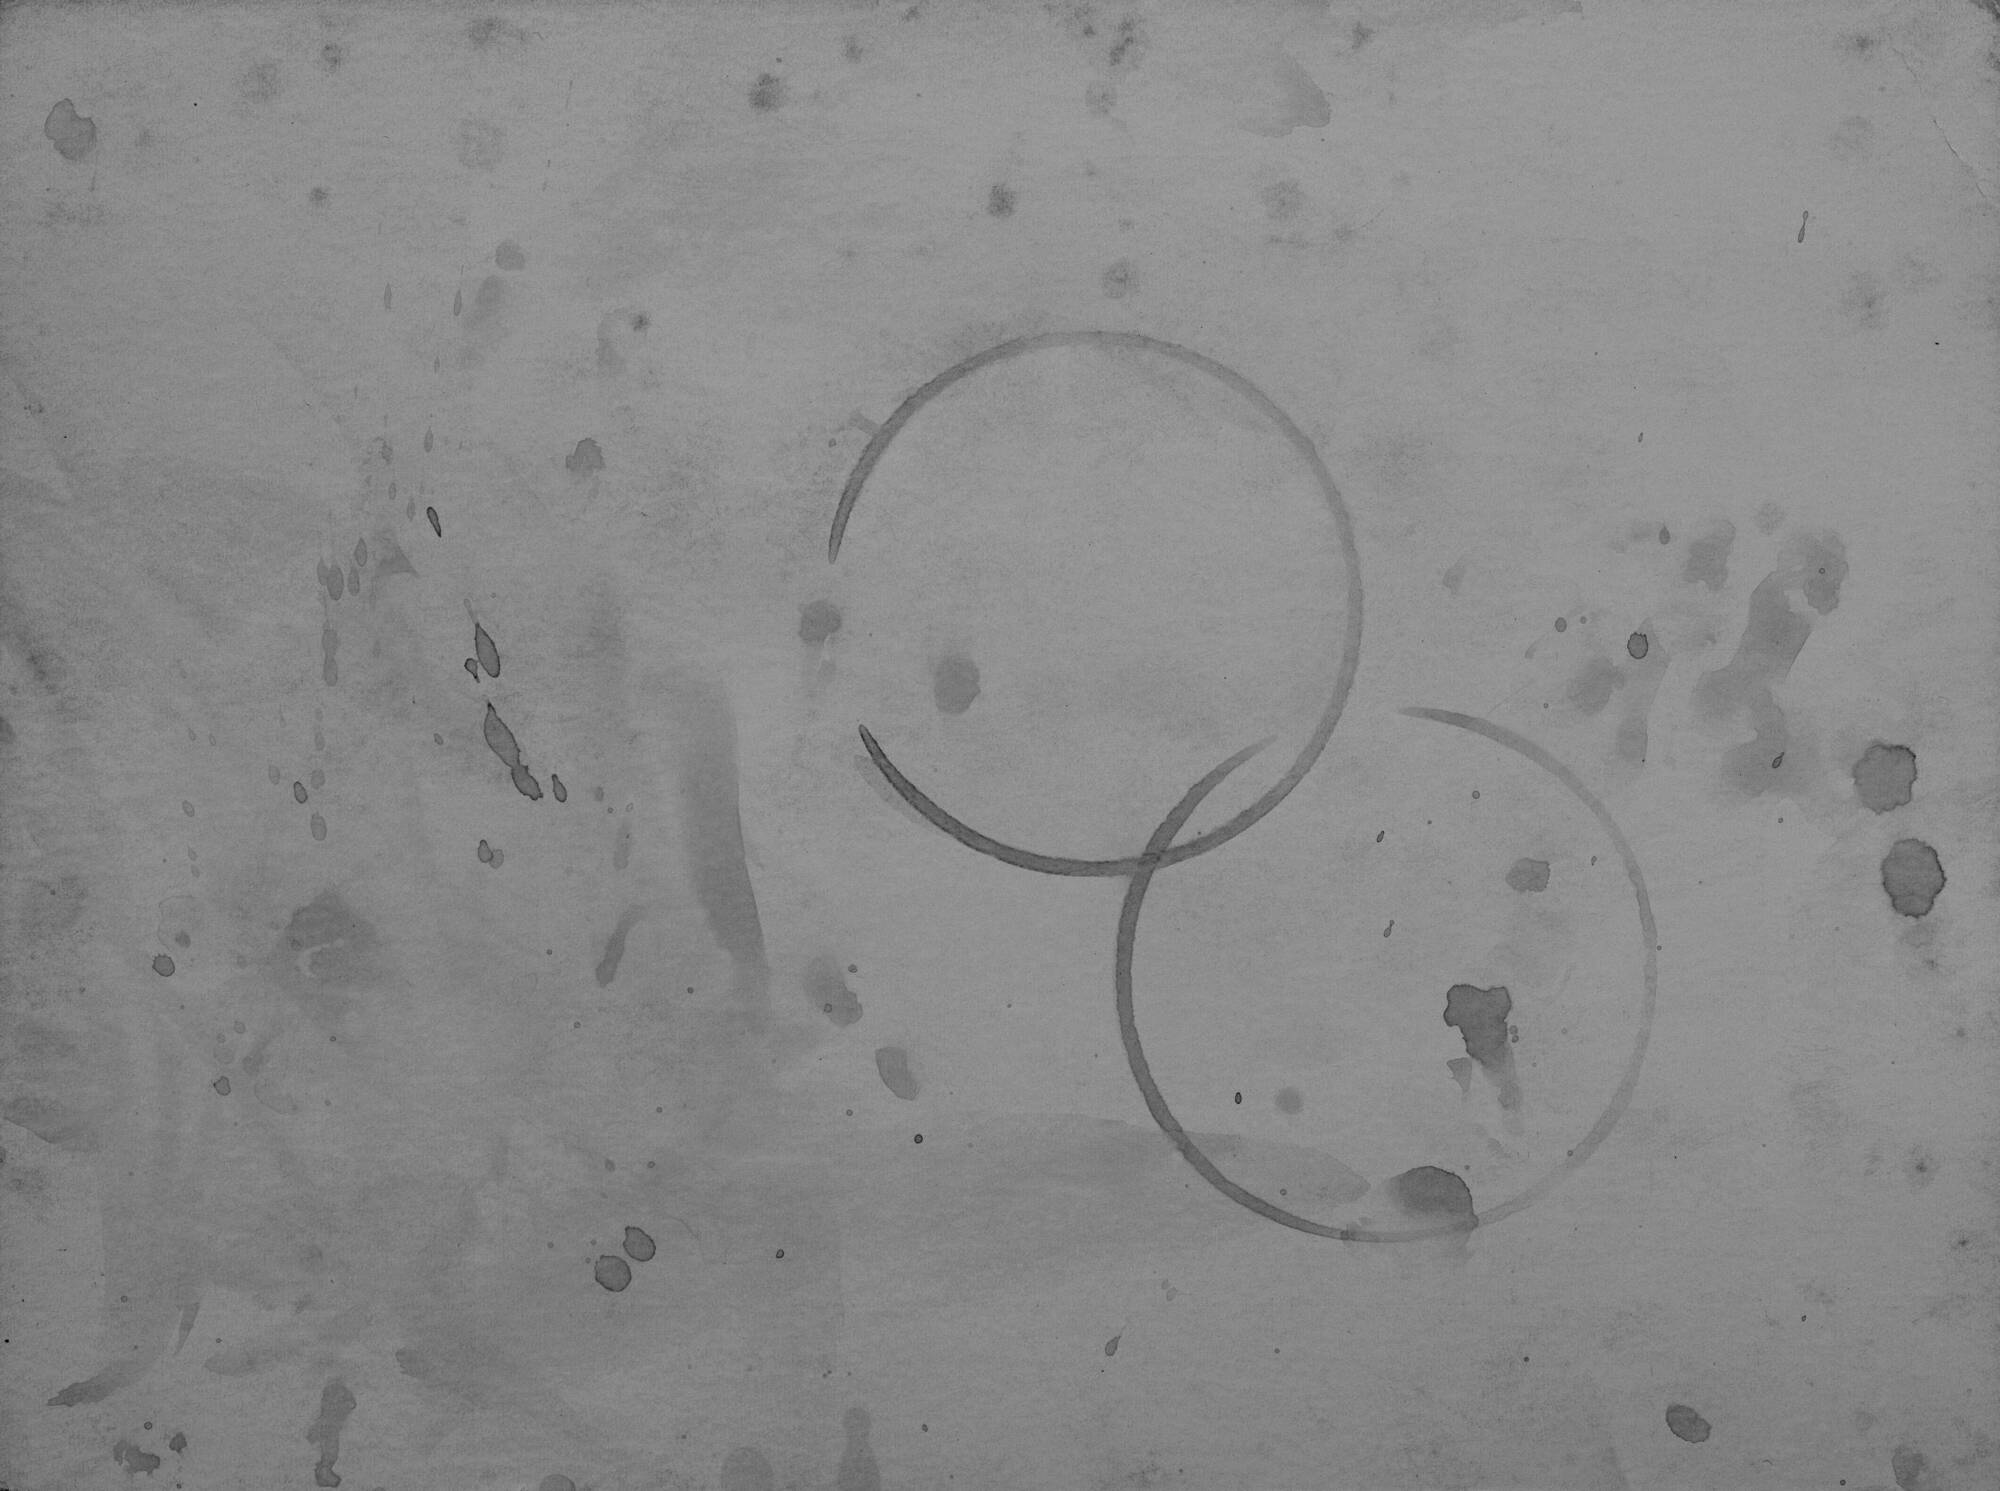
\includegraphics[width=\paperwidth,height=\paperheight]{noise4.jpg} \or
              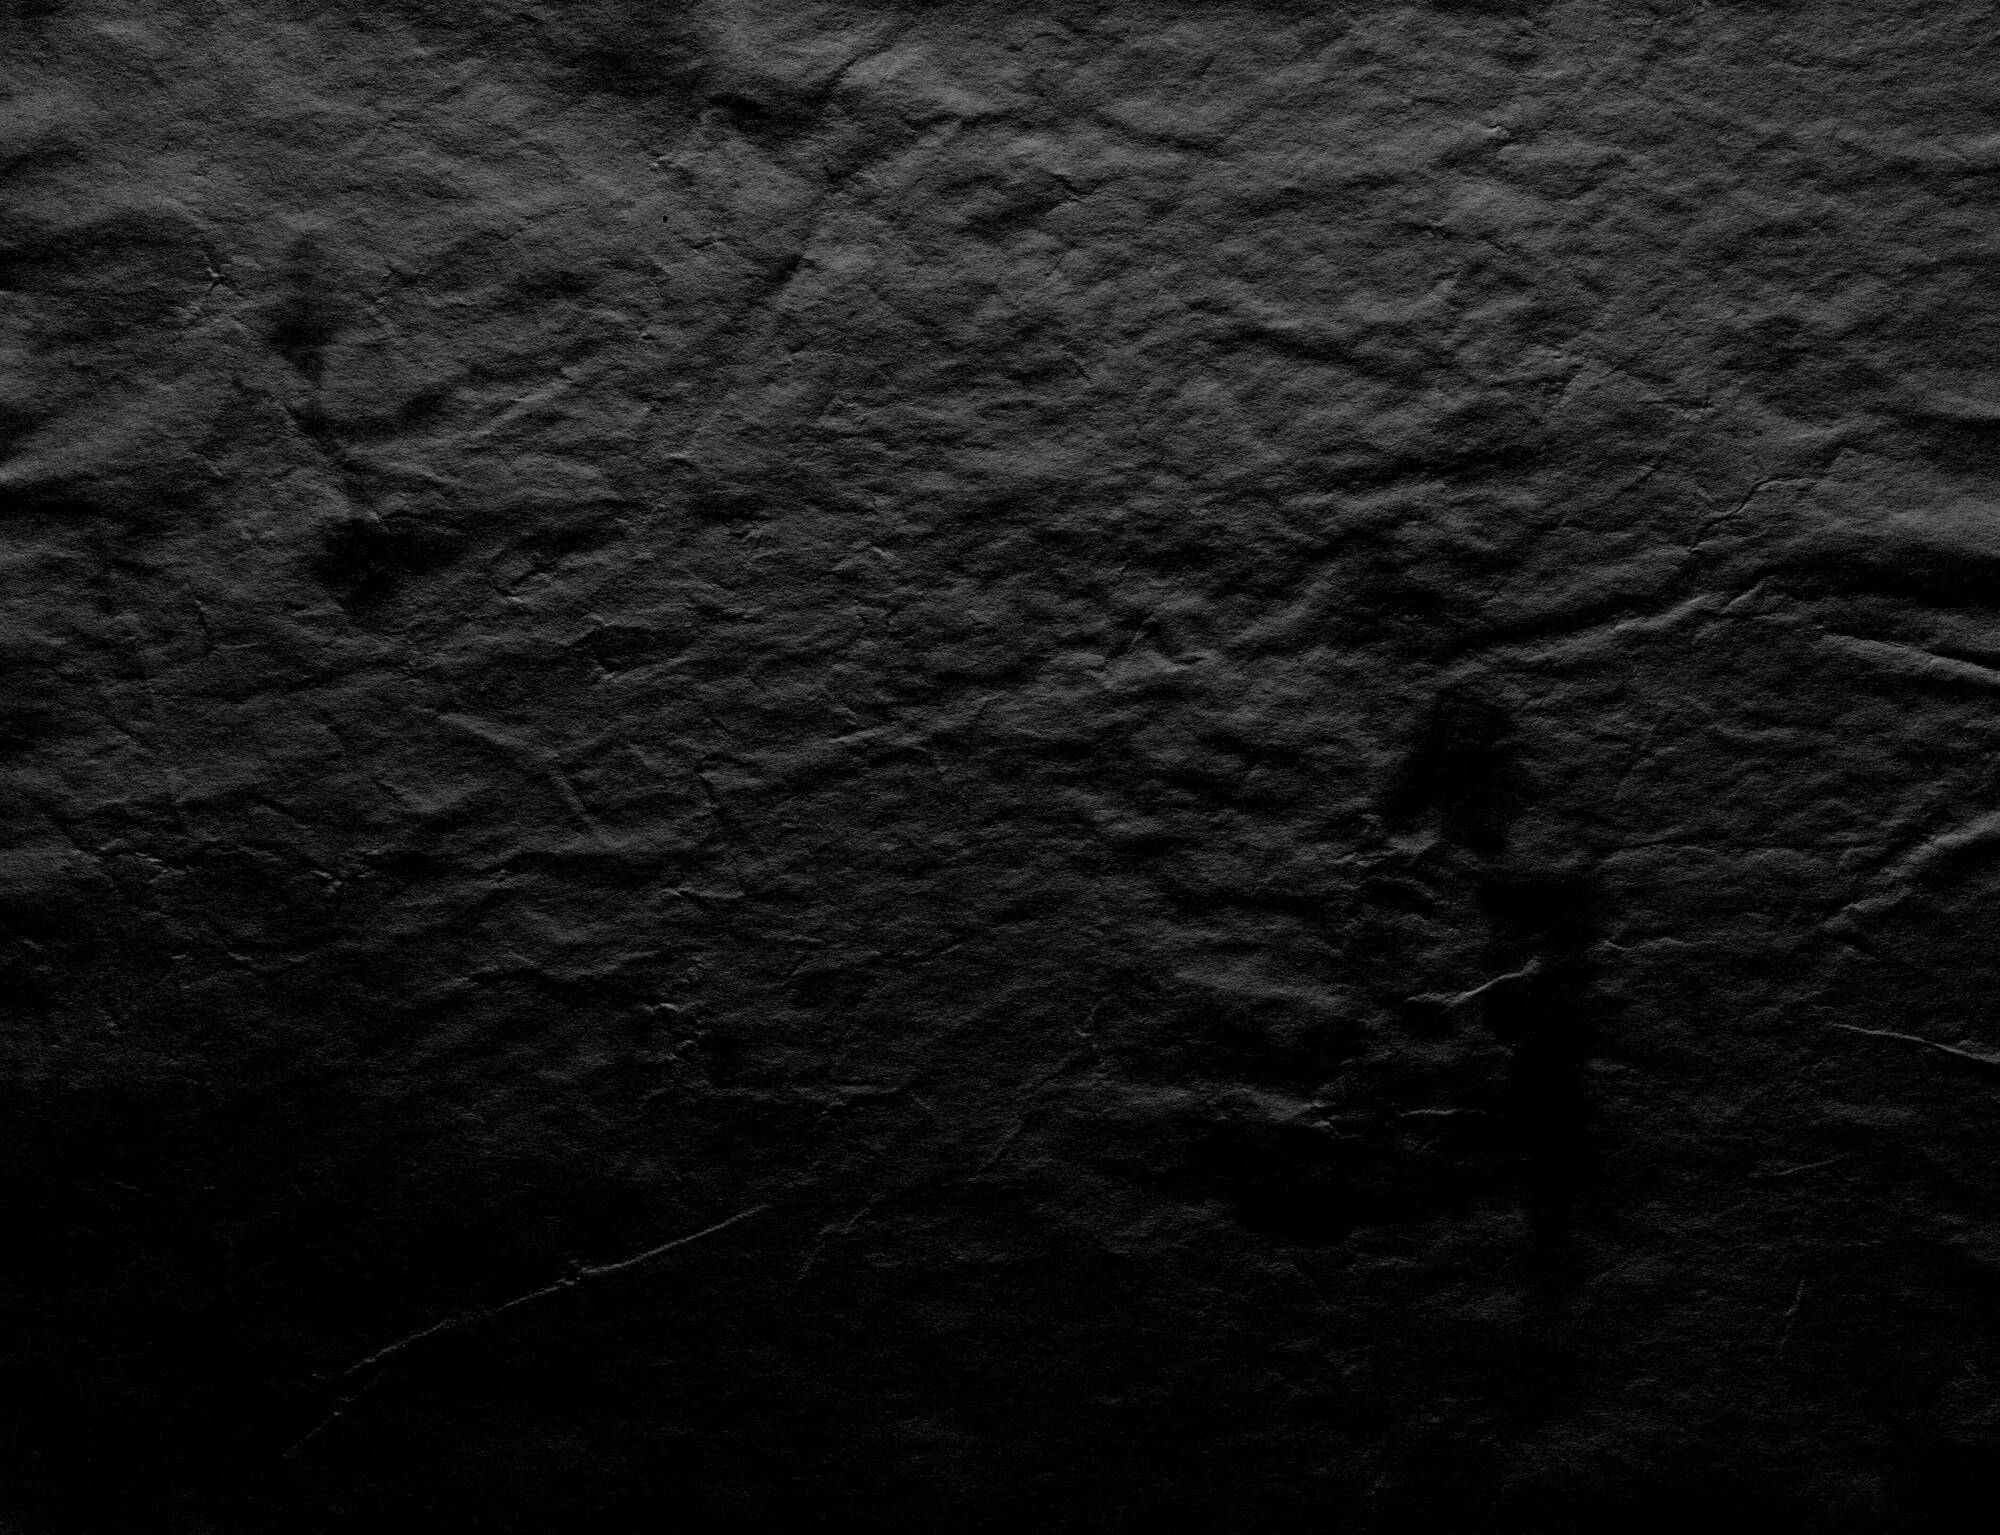
\includegraphics[width=\paperwidth,height=\paperheight]{noise5.jpg} \else
              
\includegraphics[width=\paperwidth,height=\paperheight]{noise6.jpg}
          \fi
      };
    \end{scope}
  }
}

% --- TITLE SLIDE DATA ---
\title{TITLE}

\author{\texorpdfstring{NAME 1\textsuperscript{$\dagger$} \\ 
\small Joint work with NAME 2\textsuperscript{$\dagger$} and NAME 3\textsuperscript{$\dagger$}}{}}

\institute{
\textsuperscript{$\dagger$}INSTITUTION \\
\vspace{0.5cm}
CONFERENCE}

\date{CHANGE TO DATE
    %\today
    }
\begin{document}


{\usetexture[0.04]{4} 
\setbeamercolor{background canvas}{bg=titlepagecolor} % Change 'blue!20' to your color
\begin{frame}[plain] 
    \titlepage
\end{frame}
}


\usetexture[0.1]{1}
\begin{frame}{An Equation}
    This is a slide with a grainy background.\\
There is only one box type, sketchybox. Here it is.
    \begin{sketchybox}{The Riemann Zeta Function}
    \begin{align*}
    \zeta(s) = \sum_{n\geq 1}\frac{1}{n^s} 
    \end{align*}
    for $ \Re(s)>1 $. 

\end{sketchybox}

\end{frame}


\usetexture[0.1]{2} 
\begin{frame}{Multiple sketchyboxes}
   The slides and sketchyboxes also get different backgrounds, to avoid repetition.
    \begin{sketchybox}{Continuing Zeta Analytically}
    \begin{align*}
    \zeta(s) = \frac{1}{s-1}+1-s\int_1^\infty \frac{t-\lfloor t\rfloor}{t^{s+1}}dt  
    \end{align*}
    for $ \Re(s)>0, $ $ s\neq 1. $  
     
    
    \end{sketchybox}
    \begin{sketchybox}{The Completed Zeta Function}
        \begin{align*}
        \xi(s):=s(s-1)\pi^{-s/2}\Gamma \left(\tfrac{s}{2}\right)\zeta(s) = \xi(1-s)
        \end{align*}
  is entire.
    
    \end{sketchybox}
    
    

 
\end{frame}
\usetexture[0.1]{3} 
\begin{frame}{Seeing All the Variations in sketchybox}
The background grain is taken from one of six images. Let us cycle through to see all the possibilities.
\begin{sketchybox}{Euler Product Formula $ \Re(s) >1$ }
\begin{align*}
\zeta(s) = \prod_{p\textrm{ prime}}\left(1-p^{-s}\right)^{-1}.
\end{align*}

\end{sketchybox}

\begin{sketchybox}{Zeros of Zeta}
    The zeros of zeta with $ 0<\Re(s)<1 $ are the \textit{critical} zeros. The \textit{Riemann Hypothesis} is the unproven claim that all the critical zeros of $ \zeta $ lie on the line $ \Re(s)=1/2. $  
    \end{sketchybox}

    

\end{frame}
\usetexture[0.1]{4} 
\begin{frame}{The Last sketchybox Frame}
\begin{sketchybox}{The Prime Number Theorem}
        Let $\pi(x)$ denote the prime-counting function, which gives the number of primes less than or equal to a real number $x$. As $x \to \infty$, we have the asymptotic relation:
        \begin{align*}\pi(x) \sim \frac{x}{\ln(x)}\end{align*}
        Equivalently, the limit of the quotient is given by:
        \begin{align*}\lim_{x \to \infty} \frac{\pi(x)}{x / \ln(x)} = 1.\end{align*}
    \end{sketchybox}
    
\end{frame}



\usetexture[0.1]{5} 
\begin{frame}{Yet Another Slide}
    This is another slide with a different grainy background. This slide also has a list.
    \begin{enumerate}
    \item The numbers have the same color as the title.
    \item Note that some backgrounds require less opacity
    \end{enumerate}
    


\end{frame}

\usetexture[0.1]{6} 
\begin{frame}{The Penultimate Slide}
 There are 5 different pre-loaded backgrounds. I've experimented with textures from chalkboards, metals, or fabric textures, but the best results come from vintage paper. \\

 You have to be somewhat careful with the opacity, since the textures come with their own color data that can mess with your slide's background colors.


\end{frame}

\usetexture[.15]{1}

\begin{frame}
\center
\textbf{\textcolor{maintitletext}{Thank you!}}

\end{frame}











\end{document}